\documentclass{article}
% To process a .bib file for pdflatex, you should compile your LaTeX document with the sequence: `pdflatex filename.tex`, then run `bibtex filename` (without the .bib extension), followed by two more runs of `pdflatex filename.tex`. This sequence ensures the bibliography is correctly generated and integrated into your document

% if you need to pass options to natbib, use, e.g.:
%  sort&compress option
\PassOptionsToPackage{numbers, compress}{natbib}
% before loading tackling_climate_workshop_style

% ready for submission
\usepackage{tackling_climate_workshop_style}

% to compile a preprint version, e.g., for submission to arXiv, add add the
% [preprint] option:
%     \usepackage[preprint]{tackling_climate_workshop_style}

% to compile a camera-ready version, add the [final] option, e.g.:
%     \usepackage[final]{tackling_climate_workshop_style}

% to avoid loading the natbib package, add option nonatbib:
% \usepackage[nonatbib]{tackling_climate_workshop_style}

\usepackage[utf8]{inputenc} % allow utf-8 input
\usepackage[T1]{fontenc}    % use 8-bit T1 fonts
\usepackage{hyperref}       % hyperlinks
\usepackage{url}            % simple URL typesetting
\usepackage{booktabs}       % professional-quality tables
\usepackage{amsfonts}       % blackboard math symbols
\usepackage{nicefrac}       % compact symbols for 1/2, etc.
\usepackage{microtype}      % microtypography

%%% Packages added by me
\usepackage{caption}
\usepackage{amsmath}
\usepackage{graphicx}
\usepackage{sidecap} % For side captions
\usepackage{ragged2e} % Text alignment (RaggedRight)
\usepackage{colortbl} % For coloring table cells

\title{\textit{Improving Deep Learning-Based Wildfire Smoke Plume Detection with a Multi-Model Ensemble Approach}}
% \title{\textit{A Proposal to Improve Deep Learning-Based Wildfire Smoke Plume Detection with a Multi-Model Ensemble Approach}}

% The \author macro works with any number of authors. There are two commands
% used to separate the names and addresses of multiple authors: \And and \AND.
%
% Using \And between authors leaves it to LaTeX to determine where to break the
% lines. Using \AND forces a line break at that point. So, if LaTeX puts 3 of 4
% authors names on the first line, and the last on the second line, try using
% \AND instead of \And before the third author name.

\author{%
Anonymous Author(s)
  % David S.~Hippocampus\thanks{Use footnote for providing further information
  %   about author (webpage, alternative address)---\emph{not} for acknowledging
  %   funding agencies.} \\
  % Department of Computer Science\\
  % Cranberry-Lemon University\\
  % Pittsburgh, PA 15213 \\
  % \texttt{hippo@cs.cranberry-lemon.edu} \\
  % examples of more authors
  % \And
  % Coauthor \\
  % Affiliation \\
  % Address \\
  % \texttt{email} \\
  % \AND
  % Coauthor \\
  % Affiliation \\
  % Address \\
  % \texttt{email} \\
  % \And
  % Coauthor \\
  % Affiliation \\
  % Address \\
  % \texttt{email} \\
  % \And
  % Coauthor \\
  % Affiliation \\
  % Address \\
  % \texttt{email} \\
}

\begin{document}

\maketitle

\begin{abstract}
With the increasing frequency and severity of wildfires, there is an urgent need for effective and rapid wildfire and smoke detection tools. Recent advancements in computer vision have demonstrated the potential of deep learning models, particularly neural networks, to automate the partitioning of high-resolution images into labelled segments. However, single-model approaches can struggle with generalization and accuracy in diverse conditions. To address these challenges, we propose using an ensemble of deep learning models to produce more accurate annotations of wildfire smoke plumes and their relative density (light, medium, heavy) in Geostationary Operational Environmental Satellite imagery. Our preliminary results indicate that ensemble techniques can improve performance compared to using a single model. This approach aims to provide a more reliable and accurate tool for real-time monitoring of smoke, ultimately informing fire and hazard management efforts and contributing to climate resilience and adaptation strategies.
% Broadly, this will be a valuable tool for air quality and fire hazard management in the face of worsening wildfires.\
% This proposal shows that multi-model deep learning ensembles could be used to support fire and hazard management by automating the real-time monitoring of smoke from satellite imagery.  

\end{abstract}

\section{Introduction}
Increased wildfire activity in recent years has led to a rise in smoke and particulate matter in the atmosphere, posing greater risks of respiratory illnesses and other air quality-induced health issues \citep{wildfire-risk}. Effective and timely wildfire and smoke detection tools are thus essential for supporting hazard management and mitigating risks to human health. 

The National Oceanic and Atmospheric Administration (NOAA) Geostationary Operational Environmental Satellites (GOES) provide high spatial and temporal resolution imagery of North America \citep{GOESbook}, which can be leveraged to detect the presence and density of smoke plumes. The NOAA Hazard Mapping System (HMS) Fire and Smoke Product currently relies on human analysts to annotate the presence of smoke over North America using GOES imagery \citep{hms}. However, this product is limited by the availability of human analysts and their time. Specifically, annotations are outputted only once to several times a day and usually have a delay between smoke occurance and the annotation. To address these limitations, we use the existing HMS dataset for training and leverage advancements in deep learning to automate the detection of smoke from GOES imagery. Deep learning models, particularly encoder-decoder neural networks, have shown promise in automating the semantic segmentation (labelling images on a pixel-wise basis with multiple classes) of high-resolution images \citep{cv-segmentation-review}. By automating this task, we can enable more frequent detection of smoke plumes, which will inform active wildfire monitoring and impacts to air quality.

This proposal focuses on enhancing the capability of deep learning models to detect smoke through the use of multi-model ensemble techniques. It has been shown for classification tasks that ensemble methods, which combine the predictions of multiple classifiers, can often perform better than a single classifier \citep{ensemble-ml}. Particularly, utilizing a diverse set of classifiers in an ensemble is important to achieve the improvement in performance \citep{ensemble-diversity}. Furthermore, when using neural networks, combining the predictions of multiple independently-trained models can improve generalization and detection accuracy \citep{nn-ensemble,nn-ensemble2, nn-error-ens}. In this proposal, we analyze various ensemble methods for the smoke detection task.
% This work builds multi-model ensembles that could support real-time fire management enabling the automatic monitoring of smoke from satellite imagery. 
% from abs: This approach aims to provide a more reliable and accurate tool for real-time monitoring of smoke, ultimately informing fire and hazard management efforts and contributing to climate resilience and adaptation strategies.
% \citep{nn-error-ens} demonstrated the importance of the neural networks having independent errors, or "error diversity" for the ensemble to succeed. it also provided a mathematical basis (clustering of errors) for designing ensembles that contain error diversity between the models.
% \section{Related Work}

\section{Data and Methods}
The dataset we use consists of 183,672 samples, each with three spectral channels (C01-C03) of GOES imagery paired with HMS smoke annotations (pixel-wise labels of smoke density of light, medium, or heavy) for a specific time and location. The data spans 2018-2024, and we use 2023 for validation and 2022 for testing, with the remaining years used for training. This ensures the testing and validation data is independent of the training data.

We utilize a variety of pre-developed encoder-decoder architectures that were designed for semantic segmentation contained within the Segmentation Models Pytorch library \citep{semantic}. We select architectures that include different features such as multi-scale fields-of-view and precise boundary detection \citep{dlv3p,PAN,UNetpp}, which are important for accurately detecting smoke plumes that can vary in size. Additionally, we select the best-performing single architecture and trained it with 12 different seeds to generate different initial random weights. These models are trained independently for 24 hours on 8 Nvidia P100 GPUs using the Adam optimizer, a learning rate of 1e-3, a binary cross entropy loss function, and batch size of 128. After training, each model is selected based on its best validation Intersection over Union (IoU) score (Equation \ref{overall_iou}) which quantifies the alignment between the model prediction ($ y^*_{i} $) and the ground truth ($y_{i}$).
\begin{equation} \label{overall_iou}
    \text{IoU}_{\text{overall}} = {\sum\limits_{i=\text{light}}^{\text{heavy}}|y_{i}\cap y^*_{i}|} \div {\sum\limits_{i=\text{light}}^{\text{heavy}}|y_{i}|\cup|y^*_{i}|}
\end{equation}
% We encourage you to communicate why the particular metrics you choose are relevant from a climate change perspective. For instance, if you are evaluating your machine learning model on the basis of accuracy, how does improved accuracy on a machine learning model translate to climate impact, and why is accuracy the best metric to use in this context?
% Could the IoU equation be put in the supplementary materials, for space? maybe it's more worthwile to discuss why improved IoU translates to climate impact
The ensemble method we are using in this preliminary analysis is an unweighted average of $N$ model outputs \citep{nn-ensemble2}. A schematic of this approach is shown in Figure \ref{fig:ensemble_framework}. To explore how performance improves with a variety of model combinations, we vary the number of ensemble members (1-12 models) for combinations of model architectures and initial random seeds. To our knowledge, these ensemble methods have not yet been used for wildfire smoke detection.
% \begin{figure}[h]
%     \centering
%     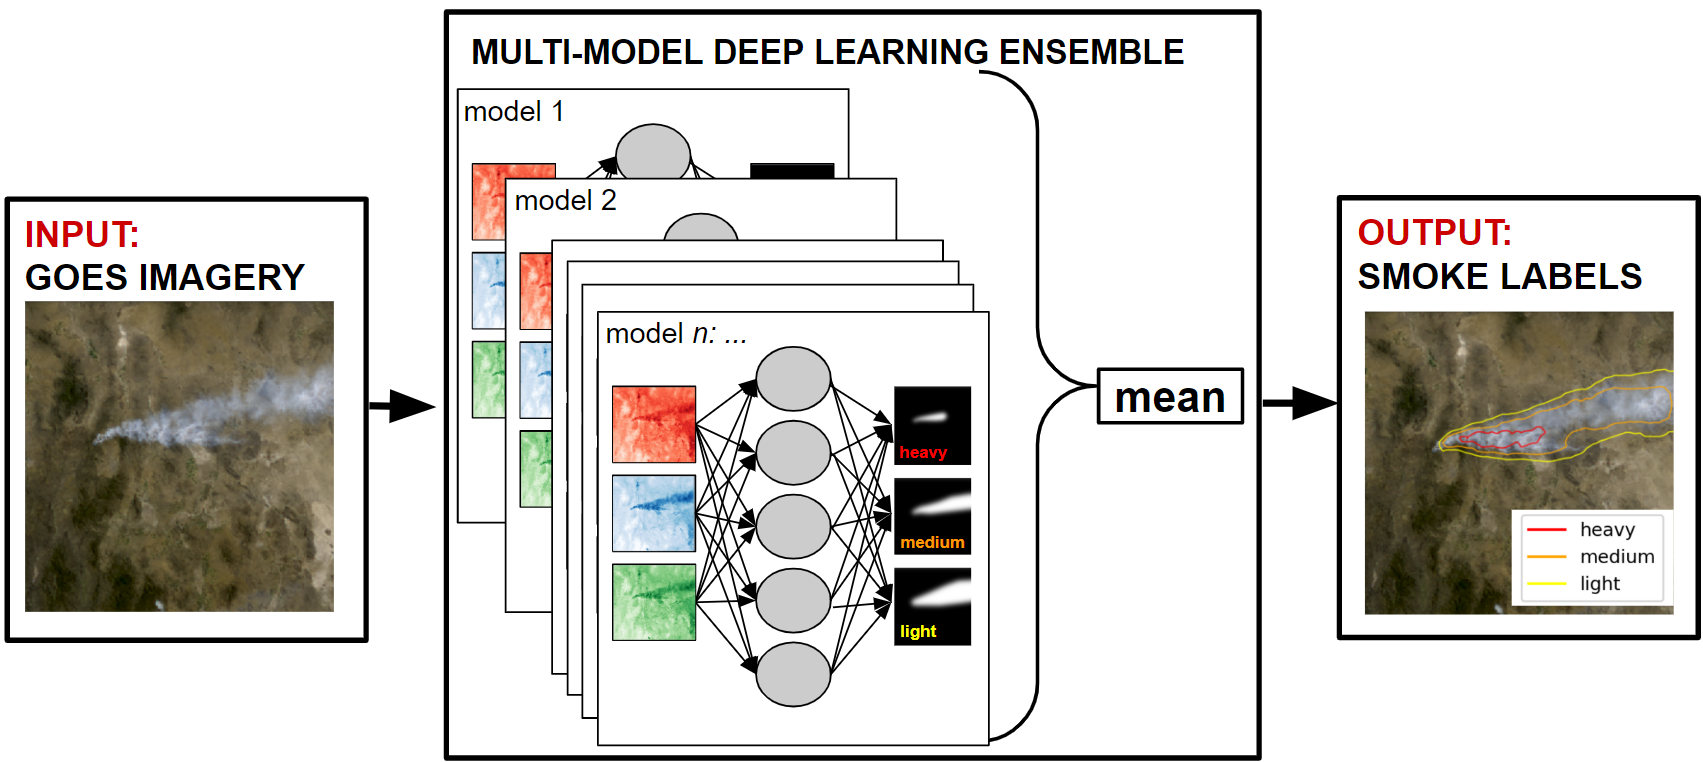
\includegraphics[width=0.7\textwidth]{ensemble_framework.png}
%     \caption{Multi-Model Ensemble Framework. GOES imagery is inputted to N independently-trained models whose output is combined with an unweighted average to produce the ensemble prediction of pixel-wise smoke labels.}
%     \label{fig:ensemble_framework}
% \end{figure}
\begin{SCfigure}[][h]
    \centering
    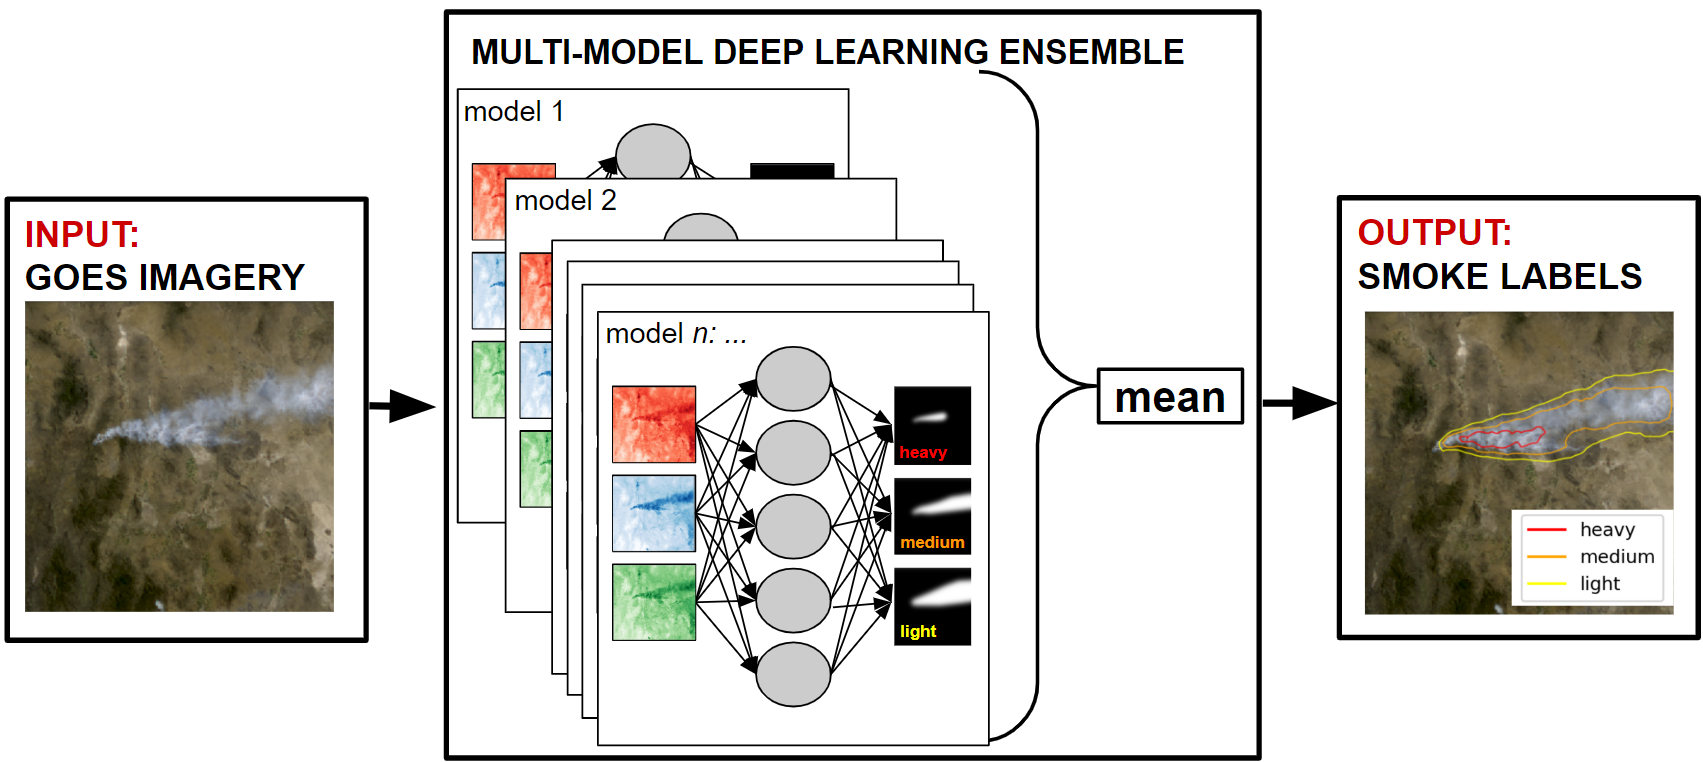
\includegraphics[width=0.7\textwidth]{ensemble_framework.png}
    \caption{\RaggedRight Multi-Model Ensemble Framework. GOES imagery is inputted to $N$ independently-trained models whose output is combined with an unweighted average to produce the ensemble prediction of pixel-wise smoke labels.}
    \label{fig:ensemble_framework}
\end{SCfigure}
\section{Results}
Table \ref{tab:results} shows the IoU scores for individual models and ensembles. The ensemble of 8 different architectures outperforms the individual models, with an improvement in the IoU score over all densities and for each density individually. The ensemble of 8 models (with the same architecure, PAN) with different initial weights also outperforms the individual models, with a similar improvement in the IoU scores. Figure \ref{fig:ensemble_size_plot} shows the IoU performance over all smoke densities as a function of ensemble size for the two ensemble schemes. The ensemble with different initial weights generally improves as models are added to the ensemble. This improvement is likely due to the different initializations leading to the models searching different parts of the parameter space and thus finding different minima of the loss function. The ensemble of different architectures improves with more models up to 8 models, but then starts to decrease in performance. This decrease in performance could be due to the additional architectures not being as well suited for the task, or the additional models not having enough variation in model bias to improve ensemble performance. Future work will aim to clarify exactly how different ensemble types and sizes reduce error and improve generalization capabilities. 
Figure \ref{fig:ensemble_panel} shows an example of smoke plume detection from the testing dataset. The ensemble predictions have smoother boundaries than the individual model outputs, making the prediction more comparable to the human-drawn polygon annotations.
\begin{table}[h]
    \centering
    \caption{IoU results across three classes of smoke (light, medium, heavy) and over all densities. Presented for different individual models of different architectures (DLV3P \citep{dlv3p}; PAN \citep{PAN}), along with the archiecture ensemble and random initial weights ensemble, where N denotes the number of models in the ensemble.}
    \label{tab:results}
    \begin{tabular}{llrrr>{\bfseries}r}
        \hline
            &   Heavy &   Medium &   Light &   Overall \\
        \hline
        Single Model: DLV3P &   0.347 &     0.441 &  0.666 &      0.599  \\
        Single Model: PAN &  0.349 &     0.478 &  0.664 &      0.604 \\
        Architecture Ensemble (N=8) &   0.400 &     0.507 &  0.692 &      0.635 \\
        %  Architecture Ensemble (N=12) &  0.400 &     0.504 &  0.686 &      0.630 \\
        Random Initial Weights Ensemble (N=8) &  0.409 &     0.512 &  0.684 &      0.631 \\
        %  Random Initial Weights Ensemble (N=12) &   0.409 &     0.515 &  0.690 &      0.635 \\
         \hline
    \end{tabular}
    \end{table}
% \begin{figure}[h]
%     \centering
%     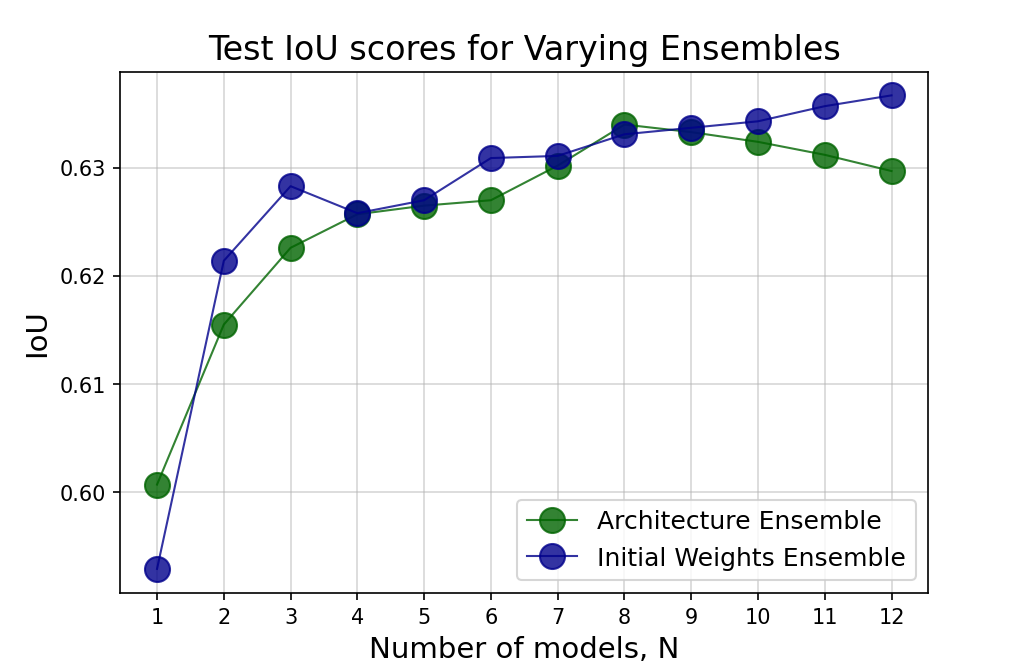
\includegraphics[width=0.70\textwidth]{ensemble_size_plot.png}
%     \caption{Ensemble IoU over all smoke densities as a function of ensemble size for two ensemble design schemes: random initial weights (blue) and architecure-based (red).}
%     \label{fig:ensemble_size_plot}
% \end{figure}
\begin{SCfigure}[][h]
    \centering
    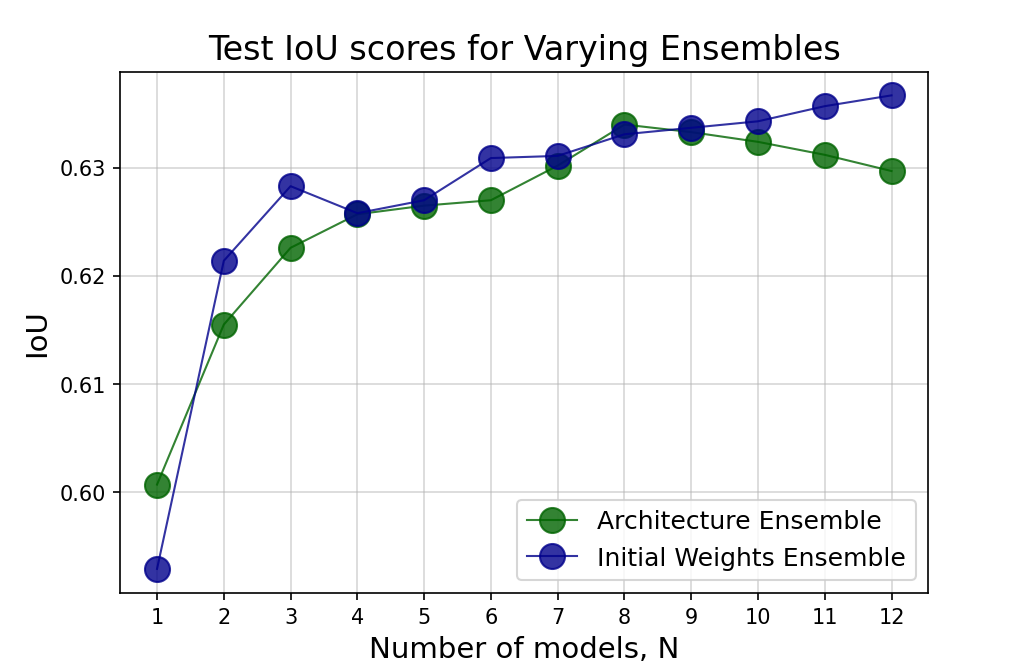
\includegraphics[width=0.70\textwidth]{ensemble_size_plot.png}
    \caption{\RaggedRight Ensemble IoU over all smoke densities as a function of ensemble size for two ensemble design schemes: random initial weights (blue) and architecure-based (red).}
    \label{fig:ensemble_size_plot}
\end{SCfigure}
\begin{figure}[h]
    \centering
    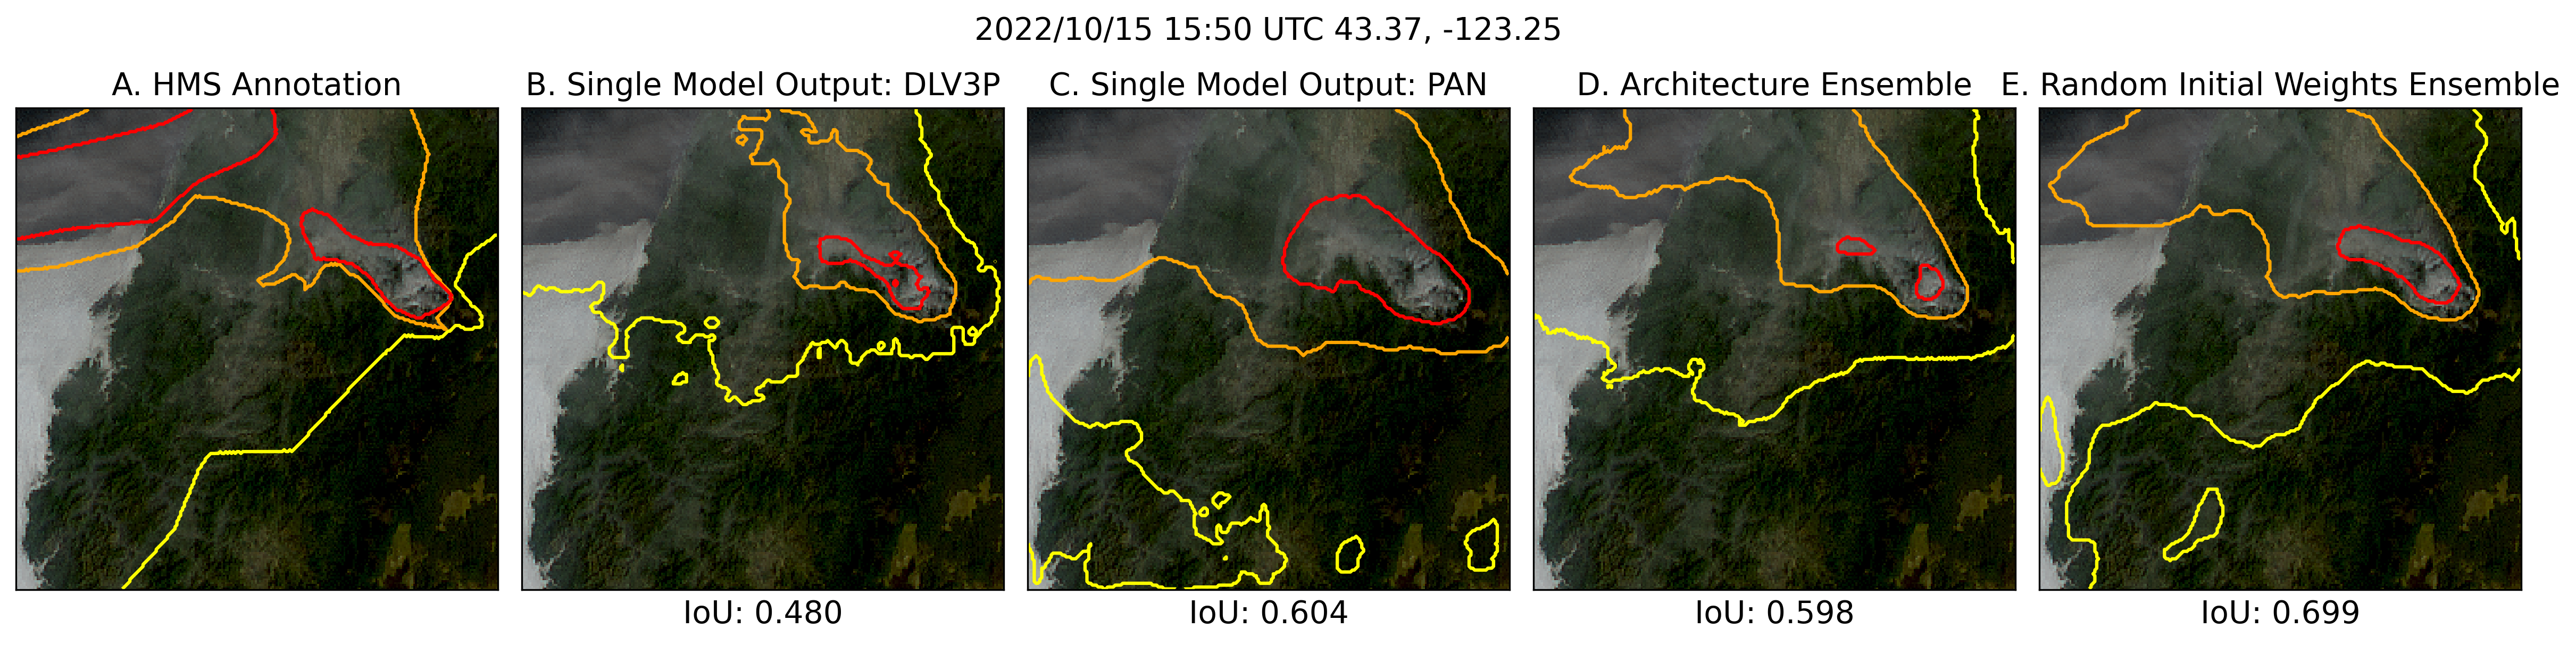
\includegraphics[width=\textwidth]{ensemble_panel_tinypaper.png}
    \caption{Example of smoke plume detection at (43.37, -123.25) on 2022/10/15 15:50 UTC. Red contours outline the heavy density smoke, orange contours outline the medium density smoke, and yellow contours outline the light density smoke annotations. Panel A displays the ground truth annotation; Panels B-C show the predictions of two individual models; Panel D shows the prediction of an architecture-based ensemble (N=8); Panel E shows the prediction of an ensemble (N=8) made with models initialized with different random weights.}
    \label{fig:ensemble_panel}
\end{figure}
\section{Conclusions and Future Work} This proposal explores two schemes for building ensembles of deep learning models that both improve on testing set IoU and smooth annotation boundaries. However, further investigation is required to understand why the architecture-based ensemble decreases in performance after 8 models, what the optimal ensemble size and type are, and exactly how the ensemble reduces error and improves generalizability. Furthermore, we plan to utilize the multi-model ensemble to quantify uncertainty in smoke annotations, enabling users like wildfire response teams and environmental agencies to assess the reliability of detections in real time. The application of these ensemble techniques are expected to aid in fire and hazard management by automating the monitoring of smoke in real-time from satellite imagery with smooth and accurate smoke annotations. This will enable improved prediction of wildfire movement and impacts to air quality, ultimately supporting climate resilience and adaptation strategies. 
% This tool can be used to provide more frequent and consistent detection of smoke plumes
\bibliographystyle{unsrt}
\bibliography{references} 

\section{Supplementary Material}
The code for this work is available at \url{https://github.com/anonymous-ensemble-smoke/ensemble-AI-smoke-detection/tree/main}. The dataset used will be released in the camera-ready version to preserve anonymity.

An additional example from the test data set is shown in Figure \ref{fig:smoothing_ex}, where the individual model output has jagged boundaries and the ensemble outputs smooth over these edges. We see a peak in performance at $N=8$ in this sample where the $N=8$ ensemble has the highest IoU score, and the smoothing does not seem to improve in the $N=12$ ensemble output. This sample supports the proposed idea that ensemble deep learning can smooth over rough edges in semantic segmentation, and warrants further investigation for the optimal ensemble size and type. 

\begin{figure}[h]
    \centering
    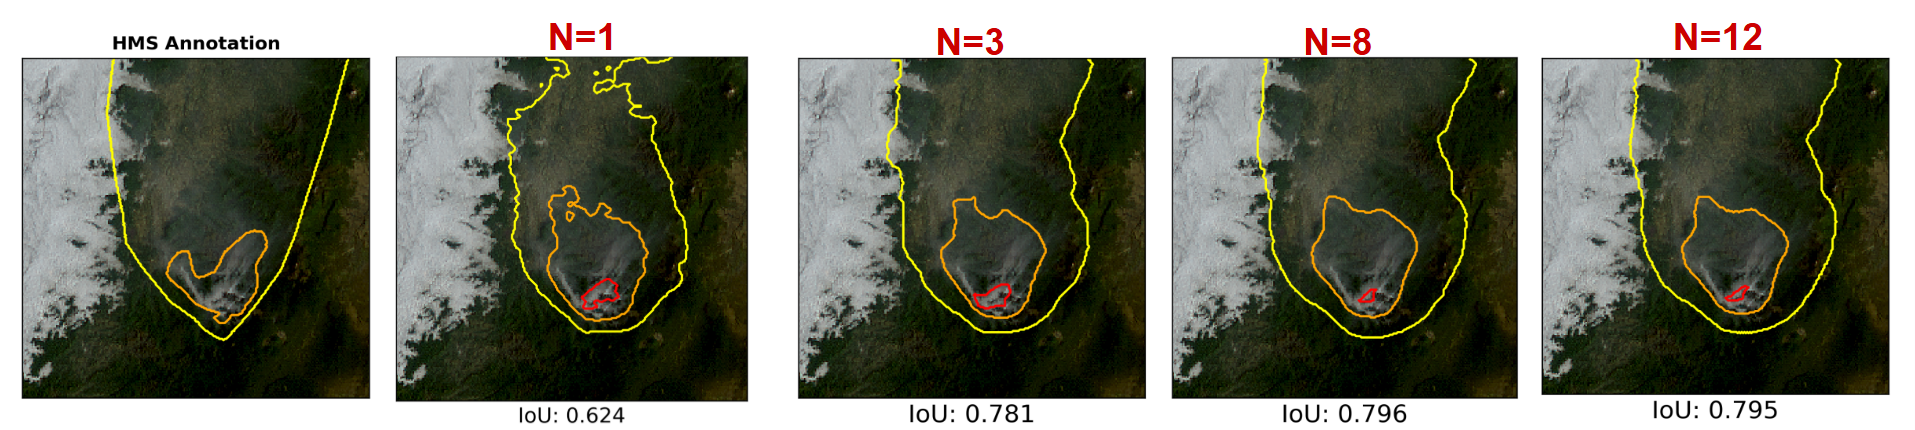
\includegraphics[width=\textwidth]{smoothing_ex.png}
    \caption{Example of smoke plume detection at (44.24, -122.74) on 2022/09/27 15:30 UTC. Red contours outline the heavy density smoke, orange contours outline the medium density smoke, and yellow contours outline the light density smoke annotations. The first panel displays the ground truth annotation; the second panel is the individual model output of DLV3P; the following panels the prediction of an architecture-based ensemble as it increases in size, $N$.}
    \label{fig:smoothing_ex}
\end{figure}

% The \LaTeX{} style file contains three optional arguments: \verb+final+, which
% creates a camera-ready copy, \verb+preprint+, which creates a preprint for
% submission to, e.g., arXiv, and \verb+nonatbib+, which will not load the
% \verb+natbib+ package for you in case of package clash.

% \paragraph{Paragraphs}

% In \LaTeX{} there is also a \verb+\paragraph+ command available, which sets the heading in bold, flush left, and inline with the text, with the heading followed by 1\,em of space. If using this style option in a \verb+docx+ file, please follow these instructions accordingly.
% would using the paragraph command save space?

% Use unnumbered first-level heading for the references. Q: what does  this mean?

% \subsection{Citations within the text}

% Citations within the text should be numbered consecutively.  The corresponding number is to appear enclosed in square brackets, such as [1] or [2]-[5].  The corresponding references are to be listed in the same order at the end of the paper, in the \textbf{References} section. (Note: the standard
% \textsc{Bib\TeX} style \texttt{unsrt} produces this.) As to the format of the references themselves, any standard reference style is acceptable, as long as it is used consistently.

% When using the \LaTeX{} template, the \verb+natbib+ package will be loaded for you by default.  Citations may be author/year or numeric, as long as you maintain internal consistency.

% For \LaTeX{} use, note that the documentation for \verb+natbib+ may be found at
% \begin{center}
%   \url{http://mirrors.ctan.org/macros/latex/contrib/natbib/natnotes.pdf}
% \end{center}
% Of note is the command \verb+\citet+, which produces citations appropriate for
% use in inline text.  For example,
% \begin{verbatim}
%    \citet{hasselmo} investigated\dots
% \end{verbatim}
% produces
% \begin{quote}
%   Hasselmo, et al.\ (1995) investigated\dots
% \end{quote}

% If you wish to load the \verb+natbib+ package with options, you may add the
% following before loading the \verb+neurips_2020+ package:
% \begin{verbatim}
%    \PassOptionsToPackage{options}{natbib}
% \end{verbatim}

% If \verb+natbib+ clashes with another package you load, you can add the optional
% argument \verb+nonatbib+ when loading the style file:
% \begin{verbatim}
%    \usepackage[nonatbib]{tackling_climate_workshop_style}
% \end{verbatim}
\end{document}